%!TEX program = xelatex
\documentclass[UTF8,zihao=5]{ctexart} %ctex包的article


\usepackage[hidelinks]{hyperref}%超链接,自动加到目录里面



\title{{\bfseries\rmfamily\Huge{DNDS 变分重构有限体积程序重整报告}}}
\author{周涵宇\hspace{2em}清华大学航天航空学院}
\date{\today}

\usepackage[a4paper]{geometry}
\geometry{left=0.75in,right=0.75in,top=1in,bottom=1in}%纸张大小和页边距

\usepackage[
UseMSWordMultipleLineSpacing,
MSWordLineSpacingMultiple=1.5
]{zhlineskip}%office风格的行间距

\usepackage{fontspec}
\setmainfont{Times New Roman}
\setsansfont{Source Sans Pro}
\setmonofont{Latin Modern Mono}
\setCJKmainfont{SimSun}[AutoFakeBold=true]
% \setCJKmainfont{仿宋}[AutoFakeBold=true]
\setCJKsansfont{黑体}[AutoFakeBold=true]
\setCJKmonofont{DengXian}[AutoFakeBold=true]

\setCJKfamilyfont{kaiti}{楷体}
\newfontfamily\CM{Cambria Math}


% \usepackage{indentfirst} %不工作 怎样调整ctex的段首缩进大小呢

\usepackage{fancyhdr}
\pagestyle{fancy}
\lhead{}
\chead{}
\rhead{}
\lfoot{}
\cfoot{\thepage}
\rfoot{}
\renewcommand{\headrulewidth}{1pt} %改为0pt即可去掉页眉下面的横线
\renewcommand{\footrulewidth}{1pt} %改为0pt即可去掉页脚上面的横线
\setcounter{page}{1}


% \usepackage{bm}

\usepackage{amsmath,amsfonts}
\usepackage{array}
\usepackage{enumitem}
\usepackage{unicode-math}

% \usepackage{titlesec} % it subverts the ctex titles
\usepackage{titletoc}


% titles in toc:
\titlecontents{section}
              [2cm]
              {\sffamily\zihao{5}\mdseries}%
              {\contentslabel{3em}}%
              {}%
              {\titlerule*[0.5pc]{-}\contentspage\hspace*{1cm}}

\titlecontents{subsection}
              [3cm]
              {\rmfamily\mdseries\zihao{5}}%
              {\contentslabel{3em}}%
              {}%
              {\titlerule*[0.5pc]{-}\contentspage\hspace*{1cm}}

\titlecontents{subsubsection}
              [4cm]
              {\rmfamily\mdseries\zihao{5}}%
              {\contentslabel{3em}}%
              {}%
              {\titlerule*[0.5pc]{-}\contentspage\hspace*{1cm}}
\renewcommand*\contentsname{\hfill \sffamily\mdseries 目录 \hfill}

\ctexset{
    section={   
        % name={前面,后面},
        number={\arabic{section}.},
        format=\sffamily\raggedright\zihao{4}\bfseries,
        indent= {0em},
        aftername = \hspace{0.5em},
        beforeskip=1ex,
        afterskip=1ex
    },
    subsection={   
        % name={另一个前面,另一个后面},
        number={\arabic{section}.\arabic{subsection}.}, %如果只用一个数字而非1.1
        format=\rmfamily\raggedright\bfseries\zihao{5},%正体字体,不加粗,main字体,五号字
        indent = {0em}, %缩进
        aftername = \hspace{0.5em},
        beforeskip=1ex,
        afterskip=1ex
    },
    subsubsection={   
        % name={另一个前面,另一个后面},
        number={\arabic{section}.\arabic{subsection}.\arabic{subsubsection}.}, %默认的 1.1.1
        format=\rmfamily\raggedright\mdseries\zihao{5},%无衬线字体,加粗,sans字体,五号字
        indent = {2em}, %缩进
        aftername = \hspace{0.5em},  %名字和标题间插入字符(此处是空白)
        beforeskip=1ex, %空行
        afterskip=1ex
    }
}

\usepackage{float}
\usepackage{graphicx}
\usepackage{multirow}
\usepackage{multicol}
\usepackage{arydshln}
\usepackage{caption}
\usepackage{subcaption}
\usepackage{cite}

\usepackage{listings}
\usepackage{xcolor-solarized}


%part、section、subsection、subsubsection、paragraph、subparagraph
\newcommand{\bm}[1]{{\mathbf{#1}}}
\newcommand{\trans}[0]{^\mathrm{T}}
\newcommand{\tran}[1]{#1^\mathrm{T}}
\newcommand{\hermi}[0]{^\mathrm{H}}
\newcommand{\conj}[1]{\overline{#1}}
\newcommand*{\av}[1]{\left\langle{#1}\right\rangle}
\newcommand*{\avld}[1]{\frac{\overline{D}#1}{Dt}}
\newcommand*{\pd}[2]{\frac{\partial #1}{\partial #2}}
\newcommand*{\pdcd}[3]{\frac{\partial^2 #1}{\partial #2 \partial #3}}
\newcommand*{\inc}[0]{{\Delta}}

\newcommand*{\uu}[0]{\bm{u}}
\newcommand*{\vv}[0]{\bm{v}}
\newcommand*{\g}[0]{\bm{g}}
\newcommand*{\nb}[0]{{\nabla}}

\newcommand*{\mean}[1]{{#1}}



\begin{document}

\maketitle
\thispagestyle{empty}
\newpage

\begin{center}
    \rmfamily
    \tableofcontents\setcounter{page}{0}
\end{center}
\thispagestyle{empty}
\newpage

% \begin{abstract} % not available in article
%     摘要
% \end{abstract}

% \chapter{DNDS:并行数值计算数据结构}

\section{DNDS:并行数值计算数据结构}

许多PDE数值方法采用区域分解进行并行计算,其好处是可以支持
极大的并行度且加速比较好。
这是因为一般PDE算法涉及的计算图是稀疏的,
即图的边数量是$O(N)$,$N$是计算的变量数量。这样,需要通信的部分只有
计算图中被区域分解切割的边。在非结构网格上,计算图的邻接关系没有规律,
因此需要一些较为麻烦的操作才能实现这样的通信。
本节主要讲述实现这些稀疏通信的基本概念。

DNDS的首要设计目标,是针对这类通信需求,
在数值设计层面尽量隐藏具体的MPI层面通信操作。
事实上,如果读者对PETSc\cite{petsc-web-page}比较熟悉,就会发现原则上这些
通信需求都可以通过Vec与IS的一些API完成。
但是在高阶格式使用中,
PETSc并不能方便地直接索引分块数据,因此就潜在地会造成
接近两倍的内存占用以及显著更大的索引开销。
例如,DNDS希望能够直接从分块稀疏矩阵中索引得到
稠密矩阵,同时方便直接操作其内存布局。
这是调用中层、上层PETSc的API不方便实现的。

%! 或许研究一下PETSc可以代替DNDS



\subsection{稀疏矩阵向量乘法}
\label{ssec:sparse_mat}

假设有一个数值向量\(V\),在典型的并行算法中其不同部分分布在不同的进程内存空间,即:
\begin{equation*}
    V = \begin{bmatrix}
        V_{[0]} \\
        V_{[1]} \\
        \dots   \\
        V_{[n_p-1]}
    \end{bmatrix}
\end{equation*}
其中\(n_p\)是进程数量。
设其维数(大小)是:\([n_0,n_1,\dots,n_{n_p-1}]\trans\),
则可以进行\(U=MV\)运算的某矩阵\(M\),有维数
\([m_0,m_1,\dots,m_{n_p-1}]\trans\times[n_0,n_1,\dots,n_{n_p-1}]\)。
本处先不论如何存储和计算这个矩阵,仅假设其输出的向量$U$
有\([m_0,m_1,\dots,m_{n_p-1}]\trans\)的维数,那么为了得到$U$,
$V$的信息必然至少经过了一定的进程间搬运。最常见的搬运方式是将每一个进程
的$U_{r}$所需的$V$的分量搬运到进程$r$,随后计算本进程的$V$,这在并行稀疏矩阵
乘向量的实现中是最常见的实现方式。这样,通过矩阵本身的稀疏邻接关系,可以
计算出哪些$V$的分量需要进行通信。此时的矩阵可以认为是一个按行分布
存储的矩阵,对于$[3,3]\times[3,3]$的矩阵,简单的例子就是:
\begin{equation}
    M=
    \left[
        \begin{array}{ccc:ccc}
            M_{00} & M_{01} &        &        &        &        \\
            M_{10} & M_{11} & M_{12} &        &        &        \\
                   & M_{21} & M_{22} & M_{23} &        &        \\
            \hline
                   &        & M_{32} & M_{33} & M_{34} &        \\
                   &        &        & M_{43} & M_{44} & M_{45} \\
                   &        &        &        & M_{54} & M_{55} \\
        \end{array}
        \right]
    \label{eq:sparseMat}
\end{equation}
这是一个稀疏的三对角矩阵,邻接图是是双向链表。
实线上下是两个进程的划分,虚线则分割了矩阵邻接关系中
指向本地和其他进程的部分。

为了方便描述具体的分量,我们定义,根据进程的编号将全局(Global)的
下标相应剖分为每个进程下的本地(Local)下标,即:
\begin{equation*}
    \begin{bmatrix}
        V_0 \\V_1\\\dots\\V_{n}
    \end{bmatrix} = \begin{bmatrix}
        V_{[0],0}             \\
        V_{[0],\dots}         \\
        V_{[0],n_0-1}         \\
        V_{[1],0}             \\
        V_{[1],\dots}         \\
        V_{[1],n_1-1}         \\
        \dots                 \\
        V_{[{n_p}],0}         \\
        V_{[{n_p}],\dots}     \\
        V_{[{n_p}],n_{n_p}-1} \\
    \end{bmatrix}
\end{equation*}
也就是说,全局编号是全局唯一的一个编号,
进程号-局部编号的整数对与全局编号一一对应。
当然,遵循这个映射规则的编号显然不唯一,但是为了方便,我们不在这里
植入任何重排,而只是采用如上文所述的顺序的编号排列。
这样的好处是,可以确定进程号-局部编号的序恰好与全局编号的序完全一致,
方便许多判断与搜索过程。这一过程是实现定义在
\verb|DNDS::GlobalOffsetsMapping|里面。
为了方便表示,默认下标是指的全局下标,任何本地的下标都可以与之简单转换。

为了实现矩阵乘法所需的通信,只需遍历$M$的局部邻接图,
找到所有非本地的指向,例如上述例子的矩阵,为$\{M_{32},M_{23}\}$,这意味着
进程$0$需要获得$V{3}$而进程$1$需要获得$V{2}$。

当然,稠密矩阵的分块存储和矩阵向量乘法需要更多的设计,比如多维分块计算等等。
但是当我们假设矩阵的稀疏性足够强,那么最简单通用的实现就是,对于需要通信的分量
直接存储到本地的虚拟(ghost)分量中,即进程$0$中$V$的ghost分量是$V_3$,
而进程$1$中其需要ghost分量$V_2$。

DNDS对于这样的ghost分量,采用拓展的本地编号,即按照编号顺序
逻辑上将所有的ghost分量排列在本地编号后面,按照上面的例子,进程
$0$中$V_3$在ghost分量的拓展本地编号是$3$,而$1$中$V_2$在
ghost分量中的拓展本地编号就是$3$。
这样,将$M$的所有分量编号转化为本地(注意第一个分量是关于$U$定义的,有时
这可能与$V$不同)则:
$$
    M=
    \left[
        \begin{array}{ccc:ccc}
            M_{00} & M_{01} &        &        &        &        \\
            M_{10} & M_{11} & M_{12} &        &        &        \\
                   & M_{21} & M_{22} & M_{23} &        &        \\
            \hline
                   &        & M_{03} & M_{00} & M_{01} &        \\
                   &        &        & M_{10} & M_{11} & M_{12} \\
                   &        &        &        & M_{21} & M_{22} \\
        \end{array}
        \right]
$$
定义拓展本地编号的好处是,假如矩阵的邻接图存储的是拓展本地编号,
矩阵向量乘法的计算索引可以看成是完全穿行的。
当然,实现中ghost部分一般按照单独的数据对象存储,那么还需要一个ghost
对象中的本地编号,对于上述示例矩阵,两个进程中的ghost本地编号都是0。

可以说,网格类算法,尤其是非结构网格中的通信结构就是以上定义的模式。
虽然说对于笛卡尔积网格(结构网格)或者说张量等数据结构也可以套用这一套计算模式,
但由于其数据索引的高度规律性,更为合理(有效率)的实现应当是对其通信模式进行
更加特殊的编码。

\subsection{从虚拟点到并行索引映射}
\label{ssec:Ghost}
虽然稀疏矩阵乘向量的需求是非结构通信的主要应用场景,但是有很多
其他的通信场合。
比如按行并行存储的稠密矩阵进行转置,
其通信需求实际上就是\verb|MPI_Alltoall|;
再比如对网格进行重分配,对于网格上定义的某个向量,
则可以理解为首先确定新网格上需要的是哪些分量编号,
随后计算本地旧网格分别需要发送到哪些进程,
以及新网格上分别需要接受哪些进程的分量,
随后进行一次\verb|MPI_Alltoallv|的通信。

事实上,这些通信需求都可以理解为一个“并行索引映射”,
或者说是将旧的向量编号搬运到新的编号位置。
\begin{equation}
    V'_{i'} := V_{i(i')}
\end{equation}
注意这个映射只要求是一个从新编号到旧编号的单射,
即$i(i')$是一个函数,
使得上式是良好定义的一个赋值运算。
也就是说原则上多个新的分量可以对应一个旧的分量。
这个定义在ghosting中就是有意义的,因为ghost向量
全局来看一般是有(在原向量意义上)重复的。

当然上述的编号映射是并行意义的,因为有$i,i'$上的新、旧
剖分$[n_0,\dots,n_{n_p}],\ [n'_0,\dots,n'_{n_p}]$定义了
新旧全局和局部编号的转换。通过这样索引的转换,
很方便定义一般的非结构通信需求。在DNDS中,我们将转换前的
向量称为father,转换后称为son。这个术语的选择可能并不是很好,
因为src和dst或许更符合习惯。但是由于father和son存在层次关系,
在思维上更接近于向量和其ghost部分的主次关系,因此DNDS的早期编写
沿用了这一术语。事实上src-dst更加合理,因为
即使存在多重的映射关系,其也是一个一般的有向图而非树。

这些编号的新旧映射计算在\verb|DNDS::OffsetAscendIndexMapping|
中实现。

\subsection{非结构二维数组 \texttt{Array}}

一般来说,稀疏矩阵可用稀疏行表达,也就是说每行只存储非零元。
对于一个每行非零元数目不一样的稀疏矩阵(或者图),那么其表示就是
一个每行不一样长的二维数组,例如对于
矩阵\ref{eq:sparseMat}中的
邻接图,就可以表示为:
\begin{equation}
    Adj_M = \begin{bmatrix}
        0 & 1 &   \\
        0 & 1 & 2 \\
        1 & 2 & 3 \\
        2 & 3 & 4 \\
        3 & 4 & 5 \\
        4 & 5 &   \\
    \end{bmatrix}
\end{equation}
注意每一行原则上是不等长的。

在非结构通信中,时常需要对邻接图本身进行通信。
一个典型的需求是,将二维表$Adj_M$的每一行理解为
向量$V$的一个分量进行通信。这样,每个进程就可以获得
本进程的节点的邻居那些行的邻接表;也就是说这样
可以知道每个本地节点的二次邻居的全局编号。
同时,网格重分配中,除了网格上定义的向量,
所有的邻接关系也需要通信。因此,有必要将
以上定义的通信模式拓展到一个二维非等长数组上。

当然,如果采用类似CGNS中的形式,大部分的邻接关系
可以分为Sections,每个Section中的等宽的二维数组。
但是DNDS方便起见优先实现了二级数组(指针数组)类型
的二维表和其CSR压缩形式,这样可以统一表示所有的
非结构邻接关系。

以上二维表具体实现为\verb|DNDS::Array|,
出于性能考虑,
对于等宽的二维表或者有最大宽度的表,其可以通过
静态设置在编译期变成静态或者等宽或者有最大宽度,
以提供相对于CSR更简单的内部索引和建立过程。

\verb|DNDS::Array|是一个纯粹的串行数据结构,
其并行的推广是\verb|DNDS::ParArray|,
概念上该对象相比于\verb|Array|要求通信器内
集体存在且拥有如\ref{ssec:sparse_mat}中
定义的全局的索引编号和索引
对象\verb|DNDS::OffsetAscendIndexMapping|。


除了邻接关系,很多计算数据也有非等宽的维度。
比如分块的Jacobian矩阵,其可以理解为一个分块稀疏矩阵,
其矩阵的稠密阵元素在每一行(对应每一个网格点)都是不等宽的。
高阶格式中很大一部分数据量就存在于这类浮点数存储中
(分块矩阵的索引部分可以极大被节省,甚至直接和网格共用邻接数据)。
这部分数据的特点是潜在地拥有更多维度,如分块稀疏的Jacobian矩阵
就是四维数组,第二个维度是边长的;而如果节点上自由度
不一定数目相等,如nodal DG方法或者精度自适应的modal DG,
第三个和第四个维度也是不相等的,原则上可以设计
带有更多维度可变长度的\verb|Array|。
但是,DNDS目前认为通信的粒度只发生在第一个维度,
因此所有后面的维度都可以被压缩为第二个维度,即,
将一行不等大小的矩阵可以压缩为一行数据。
当然,这意味可能需要存储额外的数据,比如上述
后三个维度都不均匀的四维数组,就需要额外存储后两个维度
的索引方式。\verb|Array|设计为并不管理这些数据,
而交给上层的抽象完成。典型的实现方式比如,在每一行double
数据中嵌入行内索引数据(会造成一定的数据膨胀),
或者额外附加一个整数\verb|Array|描述每一行内的索引信息。

DNDS实现了一些方便的派生\verb|ParArray|,以
存储邻接关系,
以及固定、均匀或者非均匀大小的Eigen向量以及Eigen矩阵。

\subsection{并行数组转换 \texttt{ArrayTransformer}}

上一节中的数据结构还没有涉及实际的并行数据
交换。基于\ref{ssec:Ghost}的并行索引映射概念,\\
\verb|DNDS::ArrayTransformer|就负责
将两个\verb|ParArray|进行转换。术语上,将
father的数据搬运到son之中定义为pull,反之定义为push。
逆变换在一对多的数据交换过程中会出现非良好定义的结果,
但是DNDS还是实现了这个过程以增加一定的灵活性。
默认的数据传送方向是pulling的方向。

\verb|ArrayTransformer|拥有对两个\verb|ParArray|对象的
引用,分别是father和son。\verb|ArrayTransformer|有一个
\verb|OffsetAscendIndexMapping|的引用以确定
father与son之间的索引对应关系。
在建立通信数据的过程中,\verb|ArrayTransformer|可能需要
考察father中对应行的尺寸,并且根据\verb|OffsetAscendIndexMapping|
来计算出son中每一行的尺寸。\verb|ArrayTransformer|需要将
son进行resize以匹配pulling的数据结果。这样,每一次调用
\verb|ArrayTransformer|的通信,\verb|ArrayTransformer|
就会调用MPI的通信界面进行实际的数据交换。

\subsection{实现情况}

目前DNDS实现的\verb|ArrayTransformer|
是基于非阻塞点对点MPI通信的。
由于father
中待发送数据是非连续存放,DNDS默认采用
构造\verb|MPI_Datatype|的方法隐式打包。
相比于显式打包,无需申请整个通信部分的内存,
在内存占用峰值上更小。
默认调用的是
\verb|MPI_SsendInit|
以及
\verb|MPI_RecvInit|
的持续非阻塞通信。

\verb|GlobalOffsetsMapping|以及
\verb|OffsetAscendIndexMapping|中为
计算全局与局部编号的映射分别需要进行
\verb|MPI_Allgather|以及
\verb|MPI_Alltoallv|
的聚合通信。这些通信的通信量分别在$O(n_p)$和
$O(n_{trans})$量级,其中$n_p$是进程数,
$n_{trans}$是本地需要收发的编号量。

\section{非结构网格}

\href{https://PETSc.org/release/manual/dmplex/}
{PETSc的DMPlex}对非结构网格的拓扑解释为
\href{https://en.wikipedia.org/wiki/Hasse_diagram}{Hasse图},
或者说是分层的有向无环图(DAG)。
虽然说这一表示足够一般且灵活性很高,原则上
PETSc提供的\verb|DMPlex|对象即
可以实现任何非结构网格的拓扑与场存储、转换等。
但是DNDS的实现希望其网格实现方式独立于PETSc,并且
基于具体问题能确保有最高效的索引方式。

%!说实话不一定有PETSc高效

\subsection{网格拓扑}

DNDS对非结构网格的实现是同时实现2、3维网格。
2维网格中的拓扑可以表示为:
$$
    Node\mapsto Face\mapsto Cell
$$
3维网格为:
$$
    Node\mapsto Edge \mapsto Face\mapsto Cell
$$
DNDS的网格实现对所有网格层级硬编码为以上的名称,
注意2维下的边被称作$Face$,面被称作$Cell$,
这是因为DNDS的网格需要支持2-3维统一编程,而2维网格
对应3维网格下的层级即为删除$Edge$层级。
这样唯一需要注意的是,对于板壳单元等离散概念下,
实际上的边应该用$Face$表示,实际上的面应该用$Cell$表示。
也就是说,DNDS中的$Cell$是最高的层级,而$Face$是第二高的层级,
而$Node$是最低的层级。

根据网格的(DAG),就可以确定任意两个层级间的(正向、反向)拓扑关系,
或者层级内的拓扑关系,如\verb|Cell2Node|一般是
直接给出的,\verb|Node2Cell|是逆转这个拓扑关系,
而定义中的\verb|Cell2Face|,\verb|Face2Node|这些是插值出来的。
层级内部的拓扑是无向图,是通过\verb|X2Y|以及\verb|Y2X|得到的。
例如,\verb|Cell2Cell|
可能是\verb|Cell2Face|以及\verb|Face2Cell|给出的
(这正是格心型格式的Jacobian拓扑)。
DNDS的网格使用了以上两种给出\verb|Cell2Cell|拓扑,
分别称为\verb|Cell2Cell_node|以及\verb|Cell2Cell_face|。

DNDS非结构网格默认存储\verb|Cell2Cell_node|、
\verb|Cell2Node|、\verb|Bnd2Node|、\verb|Bnd2Cell|,
其中$Bnd$是边界单元,实际上是$Face$的子集,
方便定义边界条件。为了方便格心型格式计算,提供方法
插值得到\verb|Cell2Face|、\verb|Face2Cell|、
\verb|Face2Node|。同时提供查询网格拓扑和相应信息的方法。

\begin{figure}[htbp]
    \centering
    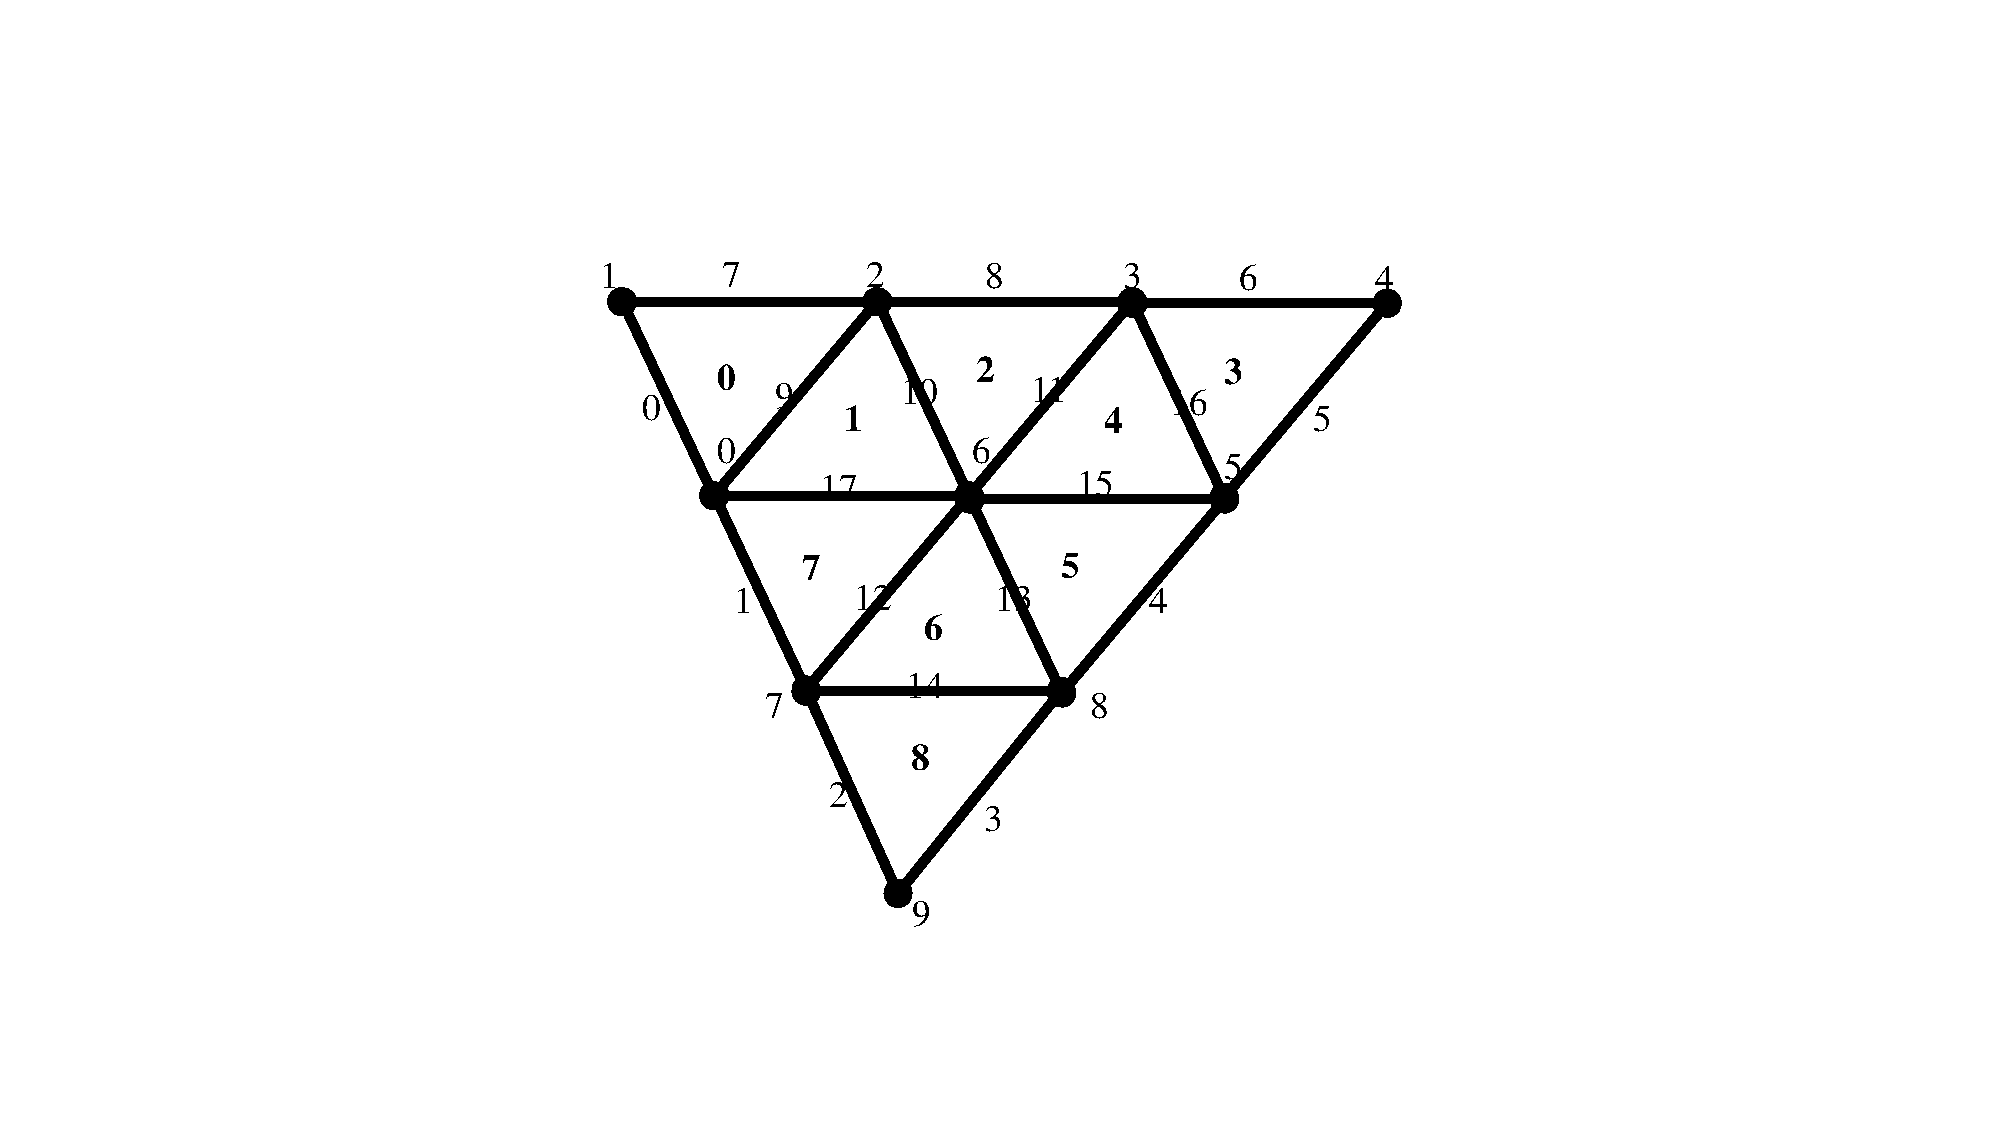
\includegraphics[width=12cm]{mesh_A.pdf}
    \caption{网格示意}
    \label{fig:mesh_A}
\end{figure}

在编号上,DNDS非结构网格目前对所有层级分别编号,
如图\ref{fig:mesh_A}即
\verb|iCell|、\verb|iFace|、\verb|iNode|是分别编号的。
并非连续编号。同时,不同层级的网格分别存储邻接关系,
存储在不同的\verb|Array|中。这样的好处是方便实现
有阶段、有选择地存储不同层级数据。

%! 或许,PETSc那种统一编号存储,也可以实现选择性构建?

以上非结构网格定义的实现在
\verb|DNDS::Geom::UnstructuredMesh|中。

\subsection{网格区域分解}

网格的任何一级都需要区域分解,
DNDS规定网格的任何一级都在全局是唯一的。
也就是说,区域分解后,全局只有唯一的$Cell$,$Node$,$Face$。
方便本地索引和计算的部分,全部存储在虚拟点上。

在并行分解过程中,划分方式(partition)可以是任意的,
当然内部实现上尽量让通信减少。$Cell$的虚拟点范围定义是,
本地可访问(即本地以及虚拟)
的$Cell$包括所有的\verb|Cell2Cell_node|邻居;
$Face$虚拟点的范围定义是,本地可访问的$Face$包含
本地\verb|Cell2Face|的全部邻居;
$Node$虚拟点的范围定义是,包含所有本地以及虚拟$Cell$
包含的$Node$。这样定义,所有本地可访问的$Cell$,
$Face$都有足够的$Node$,但是只有本地$Cell$采用足够的$Face$。

\begin{figure}[htbp]
    \centering
    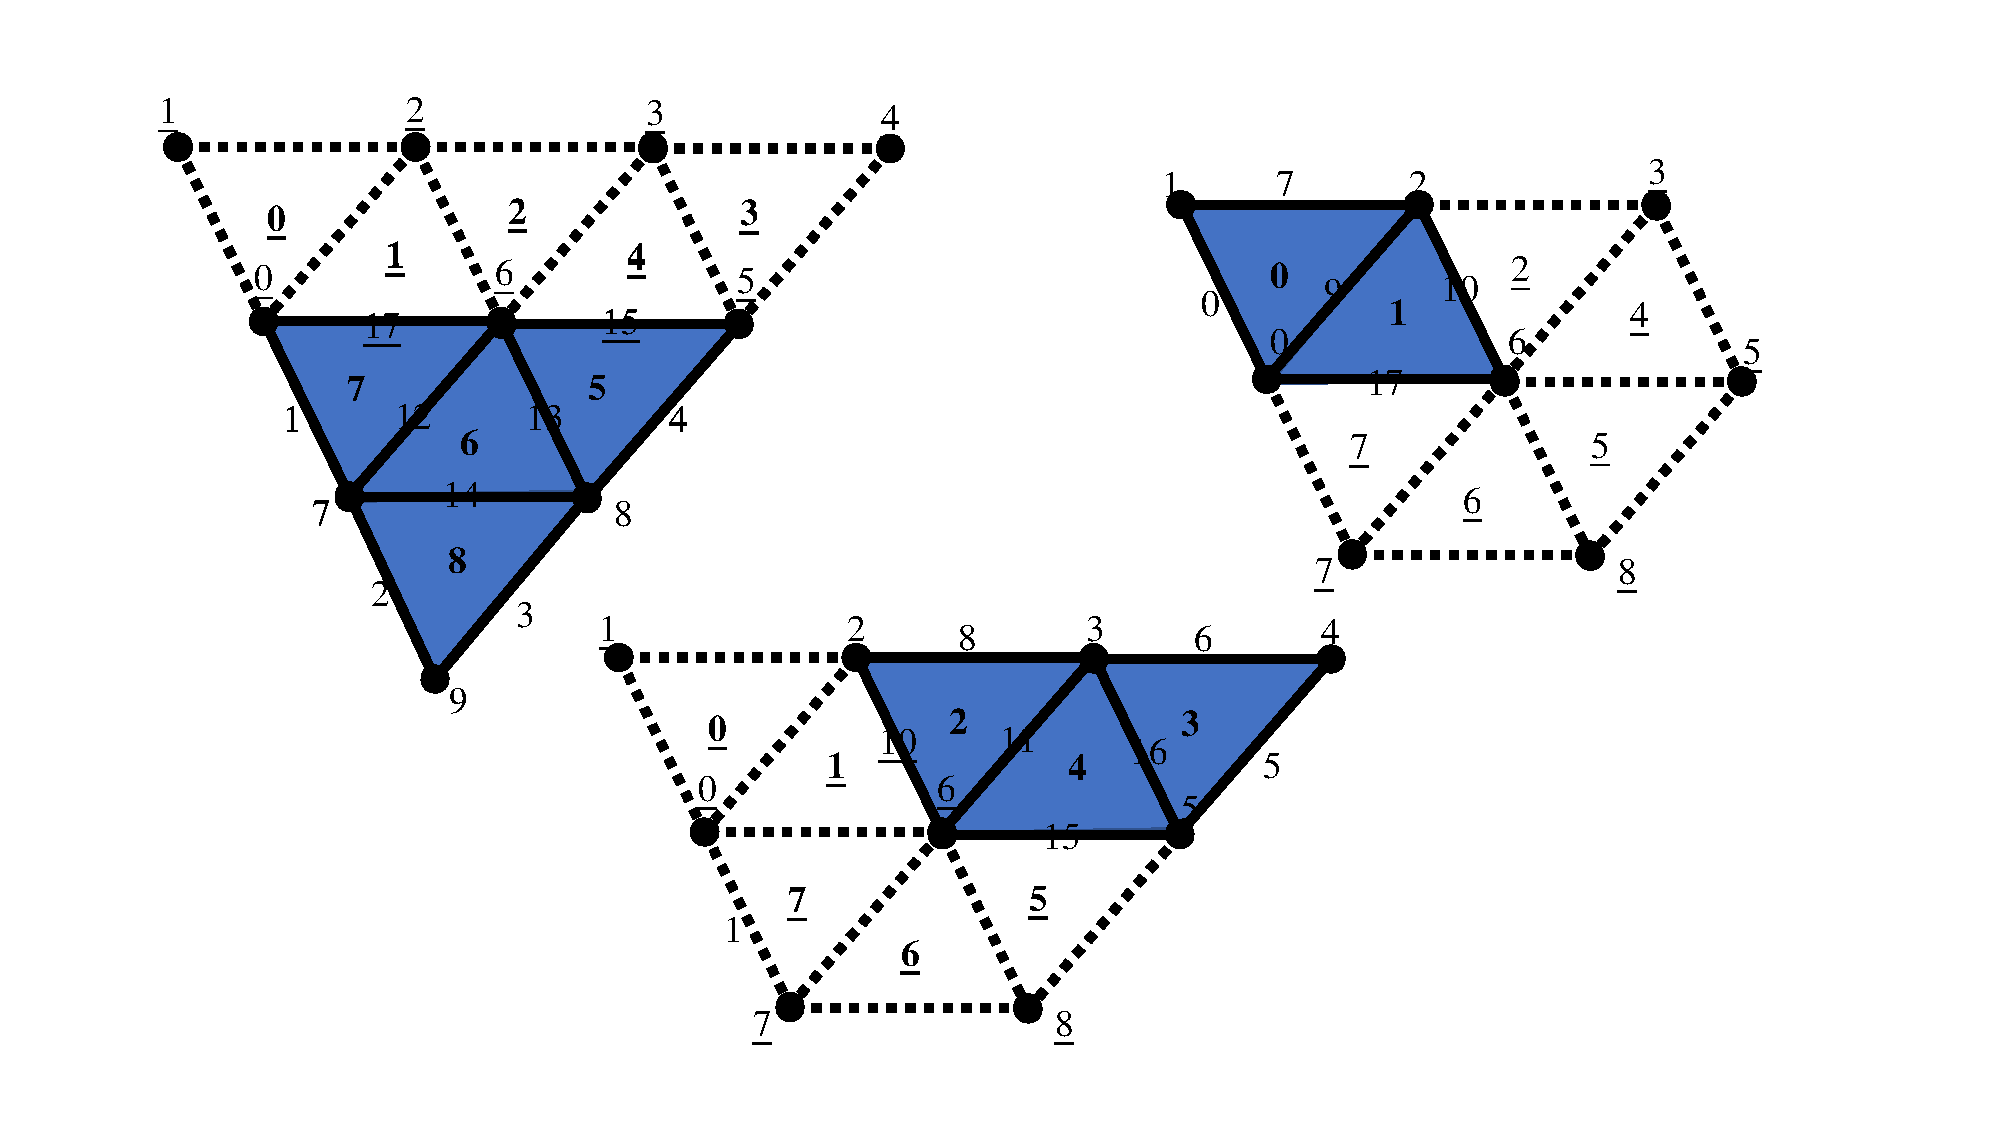
\includegraphics[width=12cm]{mesh_A_Part.pdf}
    \caption{网格剖分示意}
    \label{fig:mesh_A_Part}
\end{figure}

假如确定了$Cell$的剖分,那么$Face$的剖分可以这样确定:
在两边$Cell$的进程中,则选取进程号更小那边;$Node$同理,
采用周边$Cell$进程最小的一个。根据以上的剖分关系,
图\ref{fig:mesh_A_Part}给出了示意。
示意中,实心的单元是本地单元。
所有的编号中,存在下划线的即为虚拟点。
其中$Face$只对本地$Cell$是完整的,
虚拟$Cell$甚至可能在本地找不到面。
所有单元是唯一的。

这一套网格信息可以方便实现紧致模板的
格心型格式,如CFV,DG
等;同时基于$C^0$节点基函数的连续有限元
也容易实现。如果在对偶网格上定义格点型
有限体积等,则需要进一步给出$Edge$单元。

\subsection{网格管理实现情况}

DNDS的非结构网格管理\verb|UnstructuredMesh|
目前存储的是遵循CGNS定义的
一阶和二阶单元。
网格读取可串行读取CGNS格式
多块非结构网格,默认将其融合为单个非结构网格。
边界条件按照默认表和可定制的映射从边界名称
映射到边界编号。
边界条件不采用CGNS内置的类型。
网格支持串行、并行的可视化文件输出,
包括Tecplot二进制以及VTK ASCII格式。
场变量可在$Node$或者$Cell$输出。

网格剖分目前采用串行Metis库剖分,
基于\verb|Cell2Cell_face|邻接图。

网格支持DNDS定义的json格式持久化,
存储了必要的并行信息和网格拓扑与几何,
方便并行读写网格。

\subsection{单元插值与数值积分}

高阶格式中高阶数值积分很常用,
而高阶单元需要对应的单元插值形函数,
DNDS目前的单元管理器\verb|DNDS::Element|
硬编码了一阶和二阶单元的形函数;
积分管理器\verb|DNDS::Quadrature|
硬编码了不同参数空间内1至6阶代数精度的数值积分。
这些对象提供了抽取子单元、
积分器等接口。
使用积分器时,使用者仅需提供参数空间中
被积函数的计算方法即可。

设计上DNDS的单元和积分管理器是不依赖网格
数据结构的,可以单独提取使用。


\section{紧致有限体积变分重构}


\subsection{基于内积的变分重构表达}
\renewcommand*{\mean}[1]
{\overline{#1}}
\newcommand*{\x}[0]
{\symbf{x}}
\newcommand*{\D}[0]
{\mathcal{D}}
\newcommand*{\inner}[1]
{\left\langle#1\right\rangle}

变分重构是一个纯几何的重构过程,
与控制方程无关,可以看成一个插值算子。

单元内多项式插值为:
\begin{equation}
    \label{eq:base2rec}
    u_i(\x)=\mean{u}_i + \sum_{l=1}^{N_{base}}{u_i^l\varphi_i^l(\x)}
\end{equation}

为了求解这个多项式的待定系数,定义
一个全局泛函
\begin{equation}
    I=\sum_{F}{I_f}
\end{equation}
其中$f$是面下标。
单元界面泛函的定义是:
\begin{equation}\label{eq:IJI}
    I_f = w_g(f) \int_f{\sum_{p=0}^k{
    w_d(p)^2 \inner{\D_p(u_L)-\D_p(u_R),\D_p(u_L)-\D_p(u_R)}_{f,p}
    } d\Gamma}
\end{equation}
其中$\D_p$是一个微分算子,
将一侧的标量场$u_L, u_R$映射为
其$p$阶偏导数。这些同阶偏导数
组成的对称高维数组可以称作一系列
“准张量”,因为其在笛卡尔坐标以及
其线性变换之间满足张量的变换关系,
但在曲线坐标不满足(因此下文
给出的$\D_p$的分量都是在笛卡尔坐标或者
其线性变换内的)。可以发现,
给定多项式分布\eqref{eq:base2rec}
的标量场,$\D_p$
的分量都是$u^l_L$的线性组合。

算子$\inner{\cdot,\cdot}_{f,p}$指的是某种
对于准张量的内积,也就是说,其是准张量的一个标量函数
且对准张量的分量满足内积定义。这个内积的定义
不同可以极大影响泛函的性质。

额外的标量$w_g,w_d$分别是几何权和无量纲导数权,
分别控制不同面之间和不同导数之间权的大小变化。

这样,求解最小问题:
\begin{equation}
    [u_i^l] = \text{argmin}(I)
\end{equation}
即可得到重构系数。$[u_i^l]$指的是
逻辑上全局组装的重构系数向量。
根据$I_f$的定义,可知其一定是
$[u_i^l]$的一个多项式
\begin{equation}
    I = [u_i^l]\trans [A] [u_i^l]\trans
    - [u_i^l]\trans [b][\mean{u}_i]
\end{equation}
且全局矩阵$[A]$至少是半正定的。
假设能够保证二次项正定,存在
唯一的重构解满足线性系统:
\begin{equation} \label{eq:VREQ}
    [A] [u_i^l]\trans
    =[b][\mean{u}_i]
\end{equation}
根据泛函的具体形式,展开为局部表达就是:
\begin{equation} \label{eq:VREQ_local}
    A_{mn}^i u_i^n = \sum_{j\in S_i}{
        \left(B_{mn}^{i-j} u_j^n
        +
        b_{m}^{i-j}(\mean{u}_j - \mean{u}_i)
        \right)}
\end{equation}
其中$n$指标遵循爱因斯坦求和,$i-j$指两个单元的界面,
局部的重构系数展开为:
\begin{equation}
    \begin{aligned} \label{eq:VRCoefs}
        A_{mn}^i     & = \sum_{j\in S_i} {
        w_g(f_{i-j}) \int_{f_{i-j}}{\sum_{p=0}^k{
        w_d(p)^2 \inner{\D_p(\varphi^m_i),\D_p(\varphi^n_i)}_{f_{i-j},p}
        } d\Gamma}}                        \\
        B_{mn}^{i-j} & = {
        w_g(f_{i-j}) \int_{f_{i-j}}{\sum_{p=0}^k{
        w_d(p)^2 \inner{\D_p(\varphi^m_i),\D_p(\varphi^n_j)}_{f_{i-j},p}
        } d\Gamma}}                        \\
        b_{m}^{i-j}  & = {
        w_g(f_{i-j}) \int_{f_{i-j}}{{
        w_d(0)^2 \inner{\varphi^m_i,1}_{f_{i-j},p}
        } d\Gamma}}
    \end{aligned}
\end{equation}
这就是可以直接在程序中写入的
计算公式。

关于上述重构系统的求解,
王乾
\cite{wang2016compact,wang2016compact2,wang2017compact3}
已经充分讨论,DNDS中默认的求解重构系统方式
即为Block-Jacobi或者Block-SOR方法。

\subsection{基函数}

在代数的意义上(指不考虑系统的病态性和浮点系统的近似性),
任何完备$k$次多项式空间总是等价的。
但是计算时必须考虑系统的病态性。
多项式基的选取就需要格外注意。
在各向同性网格中,计算最简单的一种是沿轴缩放的泰勒基,
例如二维:
\begin{equation}
    [\phi_i^l] = \begin{bmatrix}
        \frac{x_1-x_{c1}}{\inc x_1}                                \\
        \frac{x_2-x_{c2}}{\inc x_2}                                \\
        (\frac{x_1-x_{c1}}{\inc x_1})^2                            \\
        (\frac{x_1-x_{c1}}{\inc x_1})(\frac{x_2-x_{c2}}{\inc x_2}) \\
        (\frac{x_2-x_{c2}}{\inc x_2})^2
    \end{bmatrix}
    -\mean{
        \begin{bmatrix}
            \frac{x_1-x_{c1}}{\inc x_1}                                \\
            \frac{x_2-x_{c2}}{\inc x_2}                                \\
            (\frac{x_1-x_{c1}}{\inc x_1})^2                            \\
            (\frac{x_1-x_{c1}}{\inc x_1})(\frac{x_2-x_{c2}}{\inc x_2}) \\
            (\frac{x_2-x_{c2}}{\inc x_2})^2
        \end{bmatrix}}
\end{equation}
注意这里的“泰勒基”是指零均值化后的泰勒基,或者说与零次基函数正交。
DNDS默认采用这样的基函数,其中$\inc x_i$选择的是
$\inc x_m = \max(|\{x_m\}_{node}-x_{cm}|)$,
也就是每个方向上单元节点坐标与中心最大的差距,
同时$x_{cm}=x_{bm}$,即基函数的中心取单元形心。
这种方案称作\verb|cellAlignedHBox|缩放的基函数。

DNDS原版程序有更多基函数选择,将会在需要的时候移植
到新的DNDS程序内。

\subsection{不同内积形式与尺度选取方案}

\subsubsection{王乾格式}

王乾格式\cite{wang2017compact3}选取:
$$
    \omega_g = \frac{1}{d_f},\ \ \omega_d(p) =  \frac{1}{p!}
$$
这个形式的无量纲导数权
将被称作阶乘导数权。
内积形式为:
$$
    \inner{\D_p(u_i),\D_p(u_j)}_{f,p}
    =d_f^{2p}
    \left([\D_p(u_i)]_{m...n}N_m... N_n\right)
    \left([\D_p(u_j)]_{m...n}N_m... N_n\right)
$$
其中$d_f$是跨界面单元中心距离,
$N_m$是面的单位法向量,
$d_f^{2p}$确保了内积的输出是无量纲的。
$[\D_p(u_j)]_{m...n}$是全局笛卡尔坐标的
导数分量。$m...n$下标使用爱因斯坦求和约定。

\subsubsection{潘建华格式}

潘建华格式\cite{jianhua2018high}选用
另外一种内积(以二维下三阶导数为例):
$$
    \begin{aligned}
        \inner{\D_3(u_i),\D_3(u_j)}_{f,3}
         & = \\
         &
        \left(\inc_{f,x}^3 D_{xxx}u_i\right)
        \left(\inc_{f,x}^3 D_{xxx}u_j\right)
        +    \\
         &
        \left(3\inc_{f,x}^2\inc_{f,y} D_{xxy}u_i\right)
        \left(3\inc_{f,x}^2\inc_{f,y} D_{xxy}u_j\right)
        +    \\
         &
        \left(3\inc_{f,y}^2\inc_{f,x} D_{xyy}u_i\right)
        \left(3\inc_{f,y}^2\inc_{f,x} D_{xyy}u_j\right)
        +    \\
         &
        \left(\inc_{f,y}^3 D_{yyy}u_i\right)
        \left(\inc_{f,y}^3 D_{yyy}u_j\right)
    \end{aligned}
$$
其中$D_{xxx}\equiv \pd{^3}{x\partial x\partial x}$。
注意$\inc_{f,x}, \inc_{f,y}$是
界面上的长度尺度选取,其选择了两边\verb|cellAlignedHBox|
向量中更大的分量作为界面的尺度。
无量纲导数权和几何权与王乾格式类似。

\subsubsection{黄乾旻格式}

黄乾旻格式\cite{huang2022high}
优化了导数权和几何权:
$$
    \omega_g = \left(\frac{S_f}{d_f}\right)^{0.5},
    \ \ \omega_d(p) =  [1, 0.5295, 0.2117, 0.2117]
$$
但是其内积形式改为了(以二维下三阶导数为例):
$$
    \begin{aligned}
        \inner{\D_3(u_i),\D_3(u_j)}_{f,3}
         & = \\
         &
        \left(d_f^3 D_{xxx}u_i\right)
        \left(d_f^3 D_{xxx}u_j\right)
        +    \\
         &
        \left(d_f^3 D_{xxy}u_i\right)
        \left(d_f^3 D_{xxy}u_j\right)
        +    \\
         &
        \left(d_f^3 D_{xyy}u_i\right)
        \left(d_f^3 D_{xyy}u_j\right)
        +    \\
         &
        \left(d_f^3 D_{yyy}u_i\right)
        \left(d_f^3 D_{yyy}u_j\right)
    \end{aligned}
$$

\subsubsection{DNDS中使用的各向同性泛函格式}

DNDS默认的各向同性泛函形式,
采用几何权为1,导数权为阶乘型,
且泛函内积为(以二维下三阶导数为例):
$$
    \begin{aligned}
        \inner{\D_3(u_i),\D_3(u_j)}_{f,3}
         & = \\
         &
        \left(d_f^3 D_{xxx}u_i\right)
        \left(d_f^3 D_{xxx}u_j\right)
        +    \\
         &
        3
        \left(d_f^3 D_{xxy}u_i\right)
        \left(d_f^3 D_{xxy}u_j\right)
        +    \\
         &
        3
        \left(d_f^3 D_{xyy}u_i\right)
        \left(d_f^3 D_{xyy}u_j\right)
        +    \\
         &
        \left(d_f^3 D_{yyy}u_i\right)
        \left(d_f^3 D_{yyy}u_j\right)
    \end{aligned}
$$
其中$d_f$选取的是两侧\verb|cellAlignedHBox|
平均的最大分量。
这与潘建华格式最为接近,
实验表明,其在正交笛卡尔网格上计算激波管等
较强间断的性能与潘建华格式差别非常小。

\subsection{限制器与间断探测器}

吴卓航(引用)给出了CWBAP型限制器,其在李万爱\cite{li2011multi,li2012multi}
的WBAP逐级限制方案上进行了改进。吴卓航CWBAP限制器
是在潘建华重构格式上实验的,
本文的DNDS各向同性格式与之相仿。

CWBAP的限制过程见吴卓航文章,本文不赘述。
本文仅指出对于一般基函数
进行二次重构的方法。

记$i,j$单元的基函数在一点$\x$的值及其导数为:
$$
    \mathfrak{D}_m{\varphi_i^l}\equiv [D_i]_{ml}
    , \mathfrak{D}_m{\varphi_j^l}\equiv [D_j]_{ml}
$$
其中$\mathfrak{D}_m$也是偏微分算符,
只不过将所有偏微分算子的分量依次排列,
例如二维下$\mathfrak{D}_1,\mathfrak{D}_2$
就是$\mathcal{D}_1$的分量,
$\mathfrak{D}_3,\mathfrak{D}_4,\mathfrak{D}_5$
就是$\mathcal{D}_2$的分量(排除对称部分)。
这样,基函数的各个导数就组成了矩阵。

二次重构的本质要求,
是多项式延拓并剔除零次部分,
其实等价于要求多项式延拓后,1阶导数
以及更高阶导数在某一点相等。
完全多项式空间的性质容易证明在某一点
各阶导数相等即可确定一个唯一的多项式变换
(首先变换为笛卡尔积和笛卡尔坐标的导数分量,则
$[D_i]_{ml},[D_j]_{ml}$都是对角线非零的上三角阵)。
因此,只要求解方程(二维三次重构为例)
$$
    \sum_{l=1}^{9}[D_i]_{ml}u_i^l =
    \sum_{l=1}^{9}[D_j]_{ml}u_j^l, \ \ m=1,...,9
$$
即可得到二次重构。
这样,无论基函数经历多么复杂的线性变换,
二次重构的过程是统一的。

实际程序中预先存储
$[D_i]^{-1}[D_j]$作为$j\rightarrow i$的
二次重构系数,反之亦然。
这个二次重构系数一定是上三角阵,
这也是逐次重构的理论基础。



\section{基于变分重构的NS方程求解器}

\subsection{气体力学}

DNDS的\verb|Euler|系列
求解器是理想气体NS方程求解器,
其热力学模型相当于是内置的理想气体模型,
粘性为牛顿本构。

DNDS在无粘通量方面实现了
Roe与HLLC通量\cite{toro2013Riemann},
其中Roe格式可选择\cite{fleischmann2020low}
中提到的大熵修正形式以及退化为Lax格式的
熵修正形式。
吴卓航使用的熵修正HLLE+通量也有实现。

粘性通量统一使用王乾
的方案\cite{wang2016compact2}。

\subsection{时间积分}

DNDS的\verb|Euler|系列求解器
调用的是泛型且多态的双时间步隐式求解器,
包括SSP-SDIRK4\cite{ferracina2008strong},
不同的BDF(包括隐式欧拉)方法,以及
显式的SSPRK3方法。
\verb|Euler|的隐式时间推进计算框架在进行显式计算时,
就要求使用者有意识地对于每一次重构迭代设置为
迭代收敛。如果进行定常计算,就退回隐式欧拉方法,
并且物理时间步是无穷大,且不进行时间推进只进行内迭代。

后续添加任何双时间步ODE方法都非常简单,
仅需进行少量代码增加。事实上,DNDS的ODE求解器
不依赖于基础数据结构\verb|Array|,
以及网格、重构和\verb|Euler|求解器的定义,
原则上任何计算问题经过适配
都可以调用DNDS的ODE求解器系列。
未来计划加入ESDIRK4方案。

\subsection{隐式方案}

DNDS的\verb|Euler|系列求解器
基于双时间步隐式时间推进,隐式时间步
都是基于只有一个未知的右手项的隐式格式。
这意味着如果一定要采用全隐式RK方法,
需要对ODE的界面进行扩展。

隐式过程求解非线性代数方程组,
框架内是基于CFL松弛的牛顿法,
牛顿法中的Jacobian通过零阶重构近似取得,
并且采用LU-SGS近似求解。
非定常问题中这样一般足够高效。
在定常问题中,目前DNDS可以使用线性GMRES进行
线性求解步的求解。
未来考虑将非线性求解器单独抽象,
实施非线性GMRES等非线性求解方案。
% [3979, 4938, 1337, 2872, 127]
% ["DNDS", "Geom", "CFV", "Euler", "Solver"]
\section{统计与测试}

\begin{figure}[htbp]
    \centering
    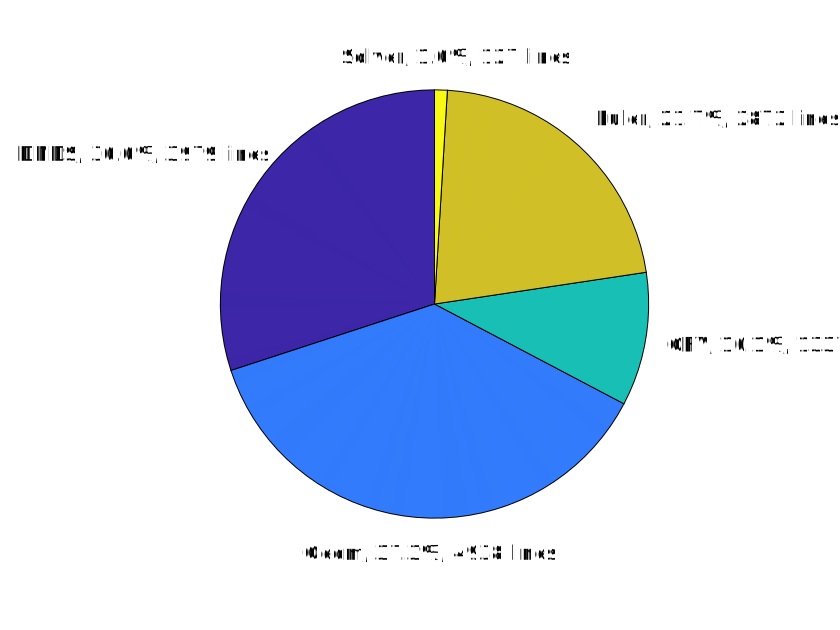
\includegraphics[width=12cm]{lines.png}  %需调整
    \caption{行数统计
        }
    \label{fig:lines}
\end{figure}

\subsection{效率与扩展性}
为了与VES程序进行直接对比,
采用双马赫反射算例LU-SGS迭代
作为评价指标。采用$h=1/480$的网格,
在TH-2B机器上使用4节点(96核)
进行计算,统计10次LU-SGS迭代的平均时间。

计算中忽略粘性项、源项,LU-SGS采用
标量Jacobian对角项进行计算,3次重构,5次积分精度。
限制器都是CWBAP,分别测试全部限制和全部不限制的方案。
%TODO

\subsection{双马赫反射}

采用吴卓航文章描述的双马赫反射算例配置,
采用笛卡尔
计算网格$h=1/240$,BDF2时间推进3200步到t=0.2,
黎曼求解器是HLLE+,采用CWBAP限制器。导数权为阶乘型,
泛函为各向同性泛函。

$t=0.2$时绘制密度从$1.41$到$22.1$的等值线30条,
如图\ref{fig:DMR}与图\ref{fig:DMR_SD}。
\ref{fig:DMR_SD}是采用间断探测器限制的结果。
图中可见,间断探测器方案与吴卓航给出的结果基本吻合。

\begin{figure}[H]
    \begin{minipage}[c]{0.45\linewidth}  %需调整
        \centering
        \includegraphics[width=8cm]{DMR.png}
        \caption{双马赫反射密度等值线,全场限制}
        \label{fig:DMR}
    \end{minipage}
    \hfill %弹性长度
    \begin{minipage}[c]{0.45\linewidth}  %需调整
        \centering
        \includegraphics[width=8cm]{DMR_SD.png}
        \caption{双马赫反射密度等值线,间断探测器限制}
        \label{fig:DMR_SD}
    \end{minipage}
\end{figure}



\subsection{三维盒子冲击}

定义三维盒子冲击问题为无粘Euler方程在
$[0,1]^3$求解,其中初始条件为盒子$[0.25,0.75]^3$
内为守恒量$(0.5,1,0,0,4)\trans$
其余为守恒量$(1,0,0,0,2.5)\trans$,计算域
边缘都是无穿透壁面。计算到$t=1$。
根据二维计算的结果,二维截面上定义的问题,
在网格尺度约小于
$1/256$时,可以明显观察到滑移面的K-H不稳定性,
其与反射的正激波作用会出现较小的涡结构。
现讨论其三维计算。

选取笛卡尔网格数$256^3$,
SDIRK4格式选用时间步$5\times10^{-4}$共2000步。
无粘通量为HLLC,施加间断探测器和限制器。
为了节省计算时间,采用3次精度的积分计算通量和重构矩阵。
由于泛函是各向同性的,
此时的重构矩阵并不会因为减少积分点而出现奇异性。

\begin{figure}[htbp]
    \centering
    \includegraphics[width=12cm]{Uniform256_3D_400_5.png}  %需调整
    \caption{三维盒子冲击问题$t=0.2$,
        曲面为$Q=0$等值面速度大小染色,
        平面为$z=0.5$密度染色}
    \label{fig:Uniform256_3D_400_5}
\end{figure}

根据特征线的限制,$t=0.2$时对称截面上的解
与二维基本一致,如图
\ref{fig:Uniform256_3D_400_5}
。
其中可见方块头尾出现明显的涡核,
而滑移面虽然还没有出现明显的
剪切失稳,Q判据已经认为三维空间中
出现一定的涡核。在经过初始的弱激波
后,涡核明显变多。

\begin{figure}[htbp]
    \centering
    \includegraphics[width=12cm]{Uniform256_3D_900_4.png}  %需调整
    \caption{三维盒子冲击问题$t=0.45$,
        曲面为$Q=0$等值面速度大小染色,
        平面为$z=0.5$密度染色}
    \label{fig:Uniform256_3D_900_4}
\end{figure}

在$t=0.45$时,如图\ref{fig:Uniform256_3D_900_4},
反射激波已经经过了滑移面的间断,
这个间断上出现了明显的二维卷起,
与二维计算基本一致。Q判据给出这几个小
卷起在三维下是条形的涡核,
与初始的大涡环平行。
此时,初始的大涡环已经在四角附近
拉伸出流向的小涡。


\begin{figure}[htbp]
    \centering
    \includegraphics[width=8cm]{Uniform256_3D_2000_1.png}  %需调整
    \caption{三维盒子冲击问题$t=1$,
        曲面为$Q=0$等值面速度大小染色,
        平面为$z=0.5$密度染色}
    \label{fig:Uniform256_3D_2000_1}
\end{figure}

\begin{figure}[htbp]
    \centering
    \subfloat[视角1]{
        \includegraphics[width=7cm]{Uniform256_3D_2000.png}
    }
    \subfloat[视角2]{
        \includegraphics[width=7cm]{Uniform256_3D_2000_2.png}
    }
    \caption{三维盒子冲击问题$t=1$,
        曲面为$Q=0$等值面速度大小染色,
        平面为$z=0.5$密度染色}
    \label{fig:Uniform256_3D_2000_2}
\end{figure}

达到$t=1$后,反射激波已经再次
在后部的壁面反射,如图\ref{fig:Uniform256_3D_2000_1}。
前面环状的涡结构围绕初始的大涡环
形成,已经发展出更多的流向涡。
图\ref{fig:Uniform256_3D_2000_2}可见
涡环附近更多的细节。
可见涡核似乎主要被限制在低密度区。
原本垂直于对称面的二维卷起涡核
已经被扭曲为三维结构。

图\ref{fig:Uniform256_3D_400_3},\ref{fig:Uniform256_3D_900_3},
\ref{fig:Uniform256_3D_1500_3},\ref{fig:Uniform256_3D_2000_3}
在同一视角绘制了$t=0.2,0.45,0.75,1$的
涡结构和密度分布。

整体上看,三维计算中计算结果确实满足三维特征,
变分重构有限体积配合限制器可以有效分辨
流动中的间断和多尺度流动结构。



\begin{figure}[htbp]
    \centering
    \includegraphics[width=12cm]{Uniform256_3D_400_3.png}  %需调整
    \caption{三维盒子冲击问题$t=0.2$,
        曲面为$Q=0$等值面速度大小染色,
        平面为$z=0.5$密度染色}
    \label{fig:Uniform256_3D_400_3}
\end{figure}

\begin{figure}[htbp]
    \centering
    \includegraphics[width=12cm]{Uniform256_3D_900_3.png}  %需调整
    \caption{三维盒子冲击问题$t=0.45$,
        曲面为$Q=0$等值面速度大小染色,
        平面为$z=0.5$密度染色}
    \label{fig:Uniform256_3D_900_3}
\end{figure}

\begin{figure}[htbp]
    \centering
    \includegraphics[width=12cm]{Uniform256_3D_1500_3.png}  %需调整
    \caption{三维盒子冲击问题$t=0.75$,
        曲面为$Q=0$等值面速度大小染色,
        平面为$z=0.5$密度染色}
    \label{fig:Uniform256_3D_1500_3}
\end{figure}

\begin{figure}[htbp]
    \centering
    \includegraphics[width=12cm]{Uniform256_3D_2000_3.png}  %需调整
    \caption{三维盒子冲击问题$t=1$,
        曲面为$Q=0$等值面速度大小染色,
        平面为$z=0.5$密度染色}
    \label{fig:Uniform256_3D_2000_3}
\end{figure}


\subsection{泰勒-格林涡}

泰勒-格林涡一般认为是不可压流动,
此处采用计算域$[0,2\pi]^3$周期边界条件,初始条件
$$
    \left\{
    \begin{array}{l}
        u = \sin(x) \cos(y) \cos(z)  \\
        v = -\cos(x) \sin(y) \cos(z) \\
        w = 0                        \\
        p = \frac{1}{\gamma M_0^2} + \frac{1}{16}\left[
            (\cos(2x) + \cos(2y)) (2 + \cos(2z))
        \right]                      \\
        \rho = \gamma M_0^2 p         \\
    \end{array}
    \right.
$$
并取$M_0=0.1$,即可近似不可压状态。
计算不加限制器,SDIRK4计算5000步到$t=10$。

在$128^3$网格计算,绘制不同时刻的涡结构如
图\ref{fig:Uniform128_3D_Periodic_TGV_5000}
。

\begin{figure}[htbp]
    \centering
    \subfloat[$t=4.6$]{
        \includegraphics[width=7cm]{Uniform128_3D_Periodic_TGV_2300.png}
    }
    \subfloat[$t=7.2$]{
        \includegraphics[width=7cm]{Uniform128_3D_Periodic_TGV_3600.png}
    }\\
    \subfloat[$t=8.0$]{
        \includegraphics[width=7cm]{Uniform128_3D_Periodic_TGV_4000.png}
    }
    \subfloat[$t=10$]{
        \includegraphics[width=7cm]{Uniform128_3D_Periodic_TGV_5000.png}
    }
    \caption{泰勒格林涡,
        曲面为$Q=0$等值面速度大小染色}
    \label{fig:Uniform128_3D_Periodic_TGV_5000}
\end{figure}

%TODO statistics





\newpage

\section*{附录}

\bibliography{refs}{}
\bibliographystyle{unsrt}


% \section*{附录}

% 本文使用的计算代码都在
% \href{https://github.com/harryzhou2000/HW_ACFD}{Github的Git Repo(点击前往)}。




















% \section{SECTION 节}

% 一个

% \subsection{SUBSECTION 小节}

% 示例

% \subsubsection{SUBSUBSECTION 小节节}

% 字体字号临时调整:
% {
%    \sffamily\bfseries\zihao{3} 哈哈哈哈哈 abcde %三号 sans系列字体(一开始设置的) 加粗
%    %只对大括号范围内的后面的字有用,在标题、题注里面同样
% }
% { 
%    \CJKfamily{kaiti}\zihao{5}\itshape 哈哈哈哈哈 abcde%三号 kaiti(一开始设置的, 斜体(英文有变)
%    %只对大括号范围内的后面的字有用,在标题、题注里面同样
% }

% 一大堆一大堆一大堆一大堆一大堆一大堆一大堆一大堆一大堆一大堆
% 一大堆一大堆一大堆一大堆一大堆一大堆一大堆一大堆一大堆一大堆一大堆一大堆
% 一大堆一大堆一大堆一大堆一大堆一大堆一大堆一大堆一大堆一大堆一大堆一大堆
% 一大堆一大堆一大堆一大堆一大堆一大堆一大堆一大堆一大堆一大堆一大堆一大堆

% \begin{center}
%     居中的什么乱七八糟东西
% \end{center}


% 一个列表:
% \begin{itemize}
%     \item asef
%     \item[\%] asdf
%     \item[\#] aaa
% \end{itemize}

% 一个有序列表:
% \begin{enumerate}
%     \item asef
%     \item[\%\%] asdf
%     \item aaa
% \end{enumerate}

% 一个嵌套列表,考虑缩进:
% \begin{enumerate}[itemindent=2em] %缩进
%     \item asef \par asaf 东西东西东西东西东西东西东西东西东西东西东西东西东西东西东西东西东西东西东西东西东西东西东西东西,
%           F不是不是不是不是不是不是不是不是不是不是不是不是不是不是不是
%           \begin{itemize}[itemindent=2em]  %缩进
%               \item lalala
%               \item mamama
%           \end{itemize}
%     \item asdf
%     \item aaa
% \end{enumerate}

% \section{SECTION}

% 图片排版:

% \begin{figure}[H]
%     \begin{minipage}[c]{0.45\linewidth}  %需调整
%         \centering
%         \includegraphics[width=8cm]{RAM_O2_4660.png}  %需调整
%         \caption{第一个图}
%         \label{fig:a}
%     \end{minipage}
%     \hfill %弹性长度
%     \begin{minipage}[c]{0.45\linewidth}  %需调整
%         \centering
%         \includegraphics[width=8cm]{RAM_O4_4660.png}  %需调整
%         \caption{第二个图}
%         \label{fig:b}
%     \end{minipage}
% \end{figure}

% figure的选项为“htbp”时,会自动浮动,是“H”则和文字顺序严格一些。

% \begin{figure}[H]
%     \begin{minipage}[c]{0.45\linewidth}  %需调整
%         \centering
%         \includegraphics[width=8cm]{RAM_O2_4660.png}  %需调整
%         \label{fig:x}
%     \end{minipage}
%     \hfill %弹性长度
%     \begin{minipage}[c]{0.45\linewidth}  %需调整
%         \centering
%         \includegraphics[width=8cm]{RAM_O4_4660.png}  %需调整
%         \label{fig:y}
%     \end{minipage}
%     \caption{第三个图}
% \end{figure}

% \begin{figure}[H]
%     \centering
%     \includegraphics[width=8cm]{RAM_O4_4660.png}  %需调整
%     \label{fig:c}
%     \caption{第四个图}
% \end{figure}



% \subsection{SUBSECTION}

% 关于怎么搞表格:

% \begin{table*}[htbp]
%     \footnotesize
%     \begin{center}
%         \caption{一端力矩载荷下的结果\fontsize{0pt}{2em}} %需要学习统一设置;0代表不变?
%         \label{表2}
%         \begin{tabular}{|c|c|c|c|c|c|c|}
%             \hline
%             节点数                              & 积分方案              & 单元数                & $h=1m$                & $h=0.1m$              & $h=0.05m$             & $h=0.01m$             \\
%             \hline
%             \multirow{6}{*}{2}                  & \multirow{3}{*}{精确} & 1                     & 4.235294117647059E-08 & 1.406250000000000E-06 & 2.862823061630218E-06 & 1.439654482924097E-05 \\
%             \cline{3-7}
%                                                 &                       & 10                    & 5.975103734439814E-08 & 4.235294117646719E-05 & 1.800000000000410E-04 & 1.406249999999849E-03 \\
%             \cline{3-7}
%                                                 &                       &
%             10000                               & 5.999999915514277E-08 & 5.999996622448291E-05 & 4.799989509752562E-04 & 5.999793702477535E-02                                                 \\
%             \cline{2-7}
%                                                 & \multirow{3}{*}{减缩} & 1                     & 6.000000000000001E-08 & 5.999999999999972E-05 & 4.799999999999911E-04 & 6.000000000003492E-02 \\
%             \cline{3-7}
%                                                 &                       & 10                    & 6.000000000000071E-08 & 5.999999999999142E-05 & 4.799999999995399E-04 & 5.999999999903294E-02 \\
%             \cline{3-7}
%                                                 &                       & 10000                 & 6.000000112649221E-08 & 5.999999234537814E-05 & 4.799997501925065E-04 & 6.000037607984510E-02 \\
%             \hline

%             \multirow{6}{*}{3}                  & \multirow{3}{*}{精确} & 1                     & 6.000000000000003E-08 & 6.000000000000202E-05 & 4.800000000000831E-04 & 6.000000000056749E-02 \\
%             \cline{3-7}
%                                                 &                       & 10                    & 5.999999999999932E-08 & 6.000000000004190E-05 & 4.800000000000206E-04 & 6.000000001613761E-02 \\
%             \cline{3-7}
%                                                 &                       & 10000                 & 6.000000013769874E-08 & 5.999989495410481E-05 & 4.799942099727246E-04 & 6.000263852944890E-02 \\
%             \cline{2-7}
%                                                 & \multirow{3}{*}{减缩} & 1                     & 6.000000000000002E-08 & 6.000000000000267E-05 & 4.800000000000754E-04 & 5.999999999989982E-02 \\
%             \cline{3-7}
%                                                 &                       & 10                    & 5.999999999999899E-08 & 5.999999999987338E-05 & 4.799999999947916E-04 & 5.999999998625345E-02 \\
%             \cline{3-7}
%                                                 &                       & 10000                 & 5.999999728157785E-08 & 5.999994914321980E-05 & 4.800008377474699E-04 & 5.999472246346305E-02 \\
%             \hline

%             \multicolumn{3}{|c|}{欧拉-伯努利解} & 6.000000000000000E-08 & 6.000000000000000E-05 & 4.800000000000000E-04 & 6.000000000000000E-02                                                 \\
%             \hline
%         \end{tabular}
%     \end{center}
% \end{table*}

% 多行、多列表格的示例,基本思想是,多列的那个东西放在多列的最上面一格,下面的行要用\&来空开,也就是\&的数目
% 和普通表格一样,是列数减一;
% 多列的部分的话,就是每行内的操作,相应的\&就少了,见最后一行。

% tabular的“|c|c|c|c|c|c|c|”,意思是,竖线-居中-竖线-居中-竖线……,可以选择省略一些竖线;
% 每行之间的hline,代表贯通的横线,cline是有范围的横线。

% \subsubsection{SUBSUBSECTION}

% newcommand可以用来定义新指令,似乎基本上就是字符串替换……不太懂,总之在公式里面可以用,
% 外面也经常用。






% 公式这么写:
% \begin{equation}
%     \begin{aligned}
%         \frac{aa(x^1+x^2)}{\sqrt{x^1x^2}}
%         \nabla\times\uu
%         = & u_{j;m}\g^m\times\g^j
%         =u_{j;m}\epsilon^{mjk}\g_k
%         =u_{j,m}\epsilon^{mjk}\g_k                           \\
%         = & \frac{1}{\sqrt{g}}\left|
%         \begin{matrix}
%             \g_1       & \g_2       & \g_3       \\
%             \partial_1 & \partial_2 & \partial_3 \\
%             u_1        & u_2        & u_3
%         \end{matrix}
%         \right|
%         =\frac{\sqrt{x^1x^2}}{aa(x^1+x^2)}
%         \left|
%         \begin{matrix}
%             \g_1                        & \g_2                        & \g_3       \\
%             \partial_1                  & \partial_2                  & \partial_3 \\
%             u^1\frac{a^2(x^1+x^2)}{x^1} & u^2\frac{a^2(x^1+x^2)}{x^2} & u^3
%         \end{matrix}
%         \right|                                              \\
%         = & \frac{\sqrt{x^1x^2}}{aa(x^1+x^2)}
%         [[\g_1\,\g_2\,\g_3]]
%         diag\left(
%         u^3_{,2}-u^2_{,3}\frac{a^2(x^1+x^2)}{x^2},\,
%         u^1_{,3}\frac{a^2(x^1+x^2)}{x^1}-u^3_{,1},\, \right. \\
%           & \left.
%         u^2_{,1}\frac{a^2(x^1+x^2)}{x^2}+u^2\frac{a^2}{x^2}
%         -
%         u^1_{,2}\frac{a^2(x^1+x^2)}{x^1}-u^1\frac{a^2}{x^1}
%         \right)                                              \\
%         = & \frac{\sqrt{x^1x^2}}{aa(x^1+x^2)}
%         [[\bm{e}_1\,\bm{e}_2\,\bm{e}_3]]
%         \left[\begin{array}{ccc} a & -a & 0\\ \frac{a\,x^{2}}{\sqrt{x^{1}\,x^{2}}} & \frac{a\,x^{1}}{\sqrt{x^{1}\,x^{2}}} & 0\\ 0 & 0 & 1 \end{array}\right]              \\
%           & diag\left(
%         u^3_{,2}-u^2_{,3}\frac{a^2(x^1+x^2)}{x^2},\,
%         u^1_{,3}\frac{a^2(x^1+x^2)}{x^1}-u^3_{,1},\, \right. \\
%           & \left.
%         u^2_{,1}\frac{a^2(x^1+x^2)}{x^2}+u^2\frac{a^2}{x^2}
%         -
%         u^1_{,2}\frac{a^2(x^1+x^2)}{x^1}-u^1\frac{a^2}{x^1}
%         \right)
%     \end{aligned}
%     \label{eq:curlu}
% \end{equation}

% 如果不想带编号的公式(或者图表),用 equation* 这种环境。

% 引用,如果是引用的图表,就用表\ref{表2},图\ref{fig:a}这种,代码里是用label定义的标签来引用,
% 编号是自动生成的。公式引用一般写成:\eqref{eq:curlu}。目前这些引用自动会有超链接,反正有那个包自动
% 好像就会有……呜呜呜也不知道是怎么做到的,先这么用吧。

% \paragraph{PARA}

% 引用文献用\\cite这些,要用bibtex,暂时不做。

% \subparagraph{SUBPARA}

\end{document}